\documentclass[11pt]{article}
\usepackage[letterpaper,margin=0.9in]{geometry}
\usepackage[hidelinks]{hyperref}
\usepackage{enumitem}
\usepackage{titlesec}
\usepackage{tabularx}
\usepackage{graphicx}

\setlist[itemize]{leftmargin=1.2em,itemsep=3pt,topsep=3pt}
\titleformat{\section}{\large\bfseries}{}{0em}{}[\titlerule]

\newcommand{\entry}[4]{
  \noindent\begin{tabularx}{\textwidth}{@{}Xr@{}}
    \textbf{#1} & #2 \\
    \textit{#3} & \textit{#4}
  \end{tabularx}\vspace{2pt}
}

\begin{document}

\noindent\begin{minipage}[t]{0.76\textwidth}
\vspace{0pt}
{\LARGE \textbf{Piter Z. Garcia Bautista}}\\[4pt]
Rochester, NY \textbar\ +1 (646) 288-3300 \textbar\ \href{mailto:pzg8794@rit.edu}{pzg8794@rit.edu}\\
\href{https://linkedin.com/in/garciapiterz}{linkedin.com/in/garciapiterz} \textbar\
\href{https://github.com/pzg8794}{github.com/pzg8794} \textbar\
\href{https://garciapiterz.com}{garciapiterz.com}
\end{minipage}%
\hfill\begin{minipage}[t]{0.20\textwidth}
\vspace{0pt}
\raggedleft
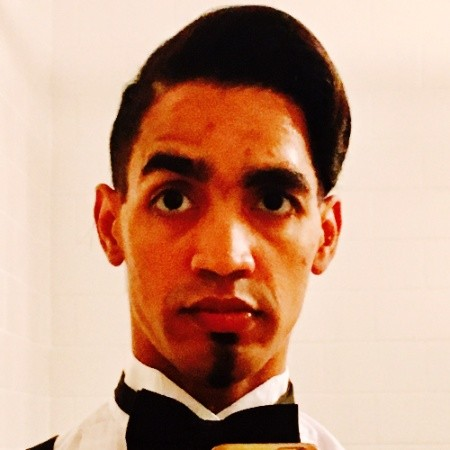
\includegraphics[width=\linewidth]{profile_pic}
\end{minipage}
\vspace{6pt}

\section{Research Profile}
Graduate researcher with a strong foundation in machine learning methods, statistical learning theory, and data-driven decision support. Background includes fairness-aware ML for high-stakes settings, reproducible evaluation frameworks, bandit and sequential decision-making algorithms, and applied ML across healthcare, bioinformatics, and network routing domains. Current Graduate Assistant work (Quantum and AI Research, RIT) emphasizes principled model evaluation, statistical rigor, and method reliability across heterogeneous and partially observed data environments. Interested in pushing ML methodology forward --- building models that generalize robustly and whose failure modes are understood and bounded.

\section{Research Interests}
Machine learning theory and methods; statistical learning and model evaluation; fairness-aware and robust ML; bandit and sequential decision-making; reproducible benchmarking; applied ML in healthcare, bioinformatics, and network systems.

\section{Education}

\entry{Rochester Institute of Technology}{Expected Aug 2026}{Master of Science, Data Science --- GPA 3.9}{Rochester, NY}
\begin{itemize}
  \item Concentration: Bioinformatics \& Artificial Intelligence.
  \item Relevant coursework: Data-Driven Knowledge Discovery (ISTE-780), Neural Networks \& Deep Learning, Applied Data Science (DSCI-601), Bioinformatics Algorithms (BIOL-630), Software Engineering for Data Science (DSCI-644), Foundations of Data Science (DSCI-633).
\end{itemize}

\entry{University of Rochester, Warner School of Education}{In progress}{Graduate study, Teaching Computer Science K--12 (M.S. track) --- GPA 4.0}{Rochester, NY}
\begin{itemize}
  \item NSF Robert Noyce Scholar (\$30,000 full funding); Advanced Certificate in Leadership in Disability and Inclusive Practices.
\end{itemize}

\entry{Rochester Institute of Technology}{2015}{Master of Science, Computer Science --- GPA 3.2}{Rochester, NY}
\begin{itemize}
  \item Concentrations: Artificial Intelligence, Big Data Analytics, Computer Graphics.
  \item Graduate research: \textit{Big Data Medical Diagnosis: A Multi-Method Approach} --- ML ensemble methods for clinical classification.
\end{itemize}

\entry{Farmingdale State College}{2012}{Bachelor of Science, Computer Engineering --- GPA 3.3}{Farmingdale, NY}
\begin{itemize}
  \item Dual degree: Electrical Engineering \& Computer Engineering Technology.
  \item Honors: CSTEP Award \& Merit; Dual BS Scholarship.
\end{itemize}

\section{Research and Professional Experience}

\entry{Rochester Institute of Technology, Software Engineering Department}{Fall 2025 -- Present}{Graduate Assistant, Quantum and AI Research}{Rochester, NY}
\begin{itemize}
  \item Build reproducible ML evaluation pipelines across local, Colab, and GCP environments with structured logging, hyperparameter tracking, and statistical validation.
  \item Develop bandit and sequential decision-making systems (UCB, neural-UCB, contextual bandits) with rigorous evaluation frameworks comparing algorithmic variants under controlled conditions.
  \item Produce manuscript-ready technical analyses on ML method performance, including evaluation under distribution shift, partial observability, and adversarial settings.
  \item Design fairness-aware evaluation protocols that measure both predictive performance and equity metrics across heterogeneous subpopulations.
\end{itemize}

\entry{University of Rochester, Warner School of Education}{Sep 2024 -- Present}{CS Teacher Candidate \& Education Research (NSF Noyce Scholar)}{Rochester, NY}
\begin{itemize}
  \item Deliver K--12 computer science instruction in active public school placement as part of the NSF Robert Noyce Scholar program, including computational thinking, inclusive pedagogy, and NYS learning standards.
  \item Conduct applied education research on AI-informed and data-driven approaches to improve learning outcomes for neurodivergent students, applying Universal Design for Learning (UDL) and evidence-based adaptive strategies.
  \item Produce lesson artifacts and instructional analyses documenting the intersection of AI, inclusive education, and evidence-based CS pedagogy.
\end{itemize}

\entry{Rochester Institute of Technology}{2024 -- 2025}{Equitable ML Research --- ISTE-780 Project (Data-Driven Knowledge Discovery)}{Rochester, NY}
\begin{itemize}
  \item Pioneered first systematic application of fairness assessment to RNA secondary structure prediction algorithms (EQUITAS framework), revealing critical equity violations (11.1\% equity score) across demographic proxies.
  \item Developed modular ML evaluation codebase (900+ lines) implementing reproducible fairness-aware algorithm comparison with automated equity-metric reporting.
  \item Achieved statistical significance ($p < 0.01$) in bias detection across multiple algorithmic variants using SHAP and disparity-impact analysis.
\end{itemize}

\entry{Rochester Institute of Technology}{2025 -- 2026}{Computational Biology Research (BIO614 and BIO550)}{Rochester, NY}
\begin{itemize}
  \item Applied ML and statistical methods to RNA structure prediction, including evaluation of probabilistic models against classical dynamic-programming baselines.
  \item Conducted RNA-seq differential-expression analysis with reproducible preprocessing, QC validation, and statistical-significance reporting.
\end{itemize}

\entry{VEDADATA Inc.}{Sep 2022 -- Aug 2024}{Data Solutions Engineer}{New York, NY}
\begin{itemize}
  \item Designed scalable Python and pandas ML workflows for ingestion, feature engineering, and statistical diagnostics in production environments.
  \item Implemented structured quality checks and anomaly-detection pipelines strengthening production data reliability.
\end{itemize}

\entry{VIOME Inc.}{Jan 2021 -- Sep 2022}{AI Data Solutions Engineer}{New York, NY}
\begin{itemize}
  \item Developed healthcare ML workflows for feature engineering, model experimentation, and evaluation --- predictive health applications in AWS production environments.
  \item Built reproducible model-evaluation infrastructure with monitoring components to detect performance degradation under distribution shift.
\end{itemize}

\section{Selected Technical Writing}
\begin{itemize}
  \item \textit{Quantum Path Optimization with Fault-Tolerant Routing} --- manuscript-level analysis of quantum-classical hybrid ML for fault-tolerant routing under noise constraints (under review, 2025--2026).
  \item \textit{Big Data Medical Diagnosis: A Multi-Method Approach} (RIT M.S.\ Computer Science graduate research, 2015) --- ensemble and deep learning methods for clinical classification on high-dimensional biomedical data.
  \item \textit{Predicting Hospital Readmission Rates: A Multi-Method ML Analysis} (DSCI-633 Project Report, 2025) --- ensemble and regularized regression methods for clinical risk stratification under distribution shift.
  \item \textit{BIO614-FinalProjectProposal} (Overleaf manuscript, 2026) --- RNA secondary structure prediction with thermodynamic deep learning enhancements, reproducible benchmarking, and biological interpretation.
  \item \textit{Equitable Bioinformatics: Enhancing Diagnostic Decision-Making through RNA and Biomarker Data} (ISTE-780 Project Report, 2025) --- fairness-aware ML for genomic diagnostic algorithms with SHAP-based bias detection and statistical significance testing.
  \item \textit{Differential Gene Expression in Murine DRG Neurons Following Sciatic Nerve Injury: An NGS Reanalysis} (BIOL550 Computational Biology Project, 2026) --- reproducible bulk RNA-seq pipeline using DESeq2, QC validation, and pathway-level biological interpretation of nociceptor gene expression.
  \item \textit{Fairness-Aware Bandits for Clinical Decision Systems} (DSCI-601 Project Proposal, 2025) --- bandit learning with equity constraints applied to high-stakes clinical diagnostic decision-making, addressing demographic disparity in sequential clinical recommendation workflows.
\end{itemize}

\section{Awards \& Recognition}
\begin{itemize}
  \item NSF Robert Noyce Teacher Scholarship (2024--2026) --- full funding for M.S. in Teaching Computer Science K--12.
  \item MS International Scholarship (2012--2015) --- MESCYT \& RIT, awarded for academic excellence.
  \item Honorable Mention Technology Award (2012) --- NYS STEP/CSTEP, 2nd place capstone project.
  \item IEEE Alumni Member (2009--Present) --- Member No. 90613000.
\end{itemize}

\section{Technical Competencies}
\textbf{Programming:} Python, R, Java, C++, C\#, SQL, MATLAB, JavaScript, Bash\\
\textbf{Machine Learning:} PyTorch, TensorFlow, scikit-learn, XGBoost; bandit/RL (UCB, contextual bandits, Thompson sampling); fairness-aware ML; model evaluation and uncertainty quantification; SHAP analysis\\
\textbf{Data and Statistics:} pandas, NumPy, SciPy, statistical modeling, hypothesis testing, reproducible benchmarking\\
\textbf{Infrastructure:} Git/GitHub, Docker, Linux, GCP, AWS, LaTeX

\section{Selected Fit for KTH Machine Learning Position}
\begin{itemize}
  \item Strong theoretical and applied ML background spanning supervised, sequential decision-making, and fairness-aware methods, with emphasis on rigorous evaluation methodology.
  \item Hands-on experience designing and running controlled ML experiments with statistical validation --- directly applicable to research that advances ML methodology.
  \item Demonstrated commitment to reproducibility: all research projects include structured evaluation pipelines, logging, and statistical-significance reporting.
  \item Deep interest in understanding when and why ML methods work or fail, with particular focus on robustness, equity, and reliability in high-stakes applications.
\end{itemize}

\end{document}
